\documentclass[20pt]{extarticle}

\usepackage[paperwidth=841mm,paperheight=1189mm,margin=22mm]{geometry}
\usepackage{fontspec}
\usepackage{graphicx}
\usepackage{ragged2e}
\usepackage{xcolor}
\usepackage{tikz}
\usetikzlibrary{arrows.meta,calc,positioning,shapes.geometric}
\usepackage[most]{tcolorbox}
\usepackage{qrcode}
\usepackage{hyperref}
\usepackage{microtype}

\setmainfont{Arial}
\setsansfont{Arial}
\renewcommand{\familydefault}{\sfdefault}
\pagestyle{empty}
\setlength{\parindent}{0pt}
\setlength{\parskip}{0pt}
\hypersetup{
  colorlinks=true,
  urlcolor=teal,
  pdftitle={The Perturbation Catalogue: An Integrated Resource for Exploring the Impact of Genetic Perturbations},
  pdfauthor={Kirill Tsukanov, Aleksandr Zakirov, Alexey Sokolov, Mallory Freeberg},
  pdfsubject={ECCB 2026 scientific poster}
}

\definecolor{Navy}{HTML}{081C2C}
\definecolor{DeepNavy}{HTML}{04131F}
\definecolor{Teal}{HTML}{006B68}
\definecolor{Emerald}{HTML}{008F67}
\definecolor{Cyan}{HTML}{2F86B7}
\definecolor{Sky}{HTML}{D9EEF3}
\definecolor{Mint}{HTML}{DDF3E8}
\definecolor{Coral}{HTML}{F0645A}
\definecolor{Gold}{HTML}{E8B44F}
\definecolor{Ink}{HTML}{13232F}
\definecolor{Slate}{HTML}{52636E}
\definecolor{Line}{HTML}{D9E2E5}
\definecolor{Paper}{HTML}{F7F9F8}
\definecolor{White}{HTML}{FFFFFF}
\pagecolor{Paper}
\color{Ink}

\newcommand{\sectionhead}[2]{%
  {\fontsize{17}{18}\selectfont\bfseries\color{#1}\MakeUppercase{#2}}\\[-1mm]
  {\color{#1}\rule{38mm}{2.3mm}}\par\vspace{4mm}}

\newcommand{\bighead}[1]{%
  {\fontsize{37}{40}\selectfont\bfseries\color{Navy}#1\par}}

\newcommand{\subhead}[1]{%
  {\fontsize{23}{27}\selectfont\color{Slate}#1\par}}

\newcommand{\pill}[2][Mint]{%
  \tikz[baseline=(p.base)]\node[
    rounded corners=5mm,fill=#1,inner xsep=5mm,inner ysep=2.2mm,
    font=\fontsize{17}{19}\selectfont\bfseries,text=Ink](p){#2};}

\newcommand{\metric}[3]{%
  \begin{tcolorbox}[
    width=\linewidth,height=55mm,enhanced,boxrule=0pt,arc=6mm,
    colback=White,left=7mm,right=7mm,top=4mm,bottom=3mm,
    borderline west={3mm}{0pt}{#1}]
    {\fontsize{39}{41}\selectfont\bfseries\color{#1}#2}\par
    \vspace{1mm}{\fontsize{17}{20}\selectfont\bfseries\color{Slate}\MakeUppercase{#3}}
  \end{tcolorbox}}

\newcommand{\stepnode}[4]{%
  \node[rounded corners=4mm,minimum width=102mm,minimum height=46mm,
        align=center,fill=#1,text=Ink,font=\fontsize{17}{19}\selectfont\bfseries] (#2) at (#4,0) {#3};}

\begin{document}
\begin{minipage}{\textwidth}

% Hero -----------------------------------------------------------------------
\begin{tikzpicture}
  \clip[rounded corners=9mm] (0,0) rectangle (\textwidth,170mm);
  \node[anchor=south west,inner sep=0] at (0,0)
    {
\includegraphics[width=\textwidth,height=170mm]{assets/hero.jpg}};
  \fill[Navy,opacity=.79] (0,0) rectangle (\textwidth,170mm);
  \fill[Teal,opacity=.32] (0,0) rectangle (430mm,170mm);
  \fill[Coral] (0,0) rectangle (\textwidth,5mm);

  \node[anchor=north west,rounded corners=4mm,fill=White,fill opacity=.94,
        text opacity=1,inner sep=5mm] at (18mm,157mm)
    {
\includegraphics[width=132mm]{assets/catalogue-logo.png}};
  \node[anchor=north east,rounded corners=5mm,draw=White,line width=.8mm,
        text=White,inner xsep=7mm,inner ysep=3.5mm,
        font=\fontsize{17}{20}\selectfont\bfseries] at ($(\textwidth,0)+(-18mm,157mm)$)
    {ECCB 2026 \;\textbullet\; GENEVA};

  \node[anchor=north west,text=White,text width=700mm,align=left,
        font=\fontsize{50}{54}\selectfont\bfseries] at (20mm,105mm)
    {The Perturbation Catalogue:\\[-1mm]
     \fontsize{42}{46}\selectfont An Integrated Resource for Exploring the Impact of Genetic Perturbations};

  \node[anchor=south west,text=White,text width=610mm,
        font=\fontsize{20}{24}\selectfont] at (21mm,25mm)
    {Kirill Tsukanov \textbullet\ Aleksandr Zakirov \textbullet\ Alexey Sokolov \textbullet\ Mallory Freeberg\\
     \fontsize{17}{21}\selectfont EMBL European Bioinformatics Institute, Wellcome Genome Campus, Hinxton, UK};

  \node[anchor=south east,rounded corners=5mm,fill=Coral,text=White,
        inner xsep=7mm,inner ysep=4mm,font=\fontsize{18}{21}\selectfont\bfseries]
        at ($(\textwidth,0)+(-18mm,15mm)$)
    {ONE SEARCH \textbullet\ THREE MODALITIES \textbullet\ COMPARABLE EVIDENCE};
\end{tikzpicture}

\vspace{7mm}

% Why ------------------------------------------------------------------------
\sectionhead{Coral}{The problem}
\bighead{A gene change is one question. The evidence is fragmented.}
\vspace{3mm}
\subhead{Different assays, formats, identifiers and processing choices make studies hard to find together---and harder to compare.}
\vspace{5mm}

\begin{tikzpicture}[x=1mm,y=1mm]
  \node[rounded corners=6mm,fill=Sky,minimum width=225mm,minimum height=60mm,
        align=left,text width=190mm,inner sep=9mm] (ps) at (115,40)
    {{\fontsize{26}{29}\selectfont\bfseries\color{Cyan}Perturb-Seq}\par
     \vspace{2mm}{\fontsize{18}{22}\selectfont Transcriptome-wide response\\Single cells \textbullet\ DEA \textbullet\ GSEA}};
  \node[rounded corners=6mm,fill=Mint,minimum width=225mm,minimum height=60mm,
        align=left,text width=190mm,inner sep=9mm] (crispr) at (389,40)
    {{\fontsize{26}{29}\selectfont\bfseries\color{Emerald}CRISPR screens}\par
     \vspace{2mm}{\fontsize{18}{22}\selectfont Gene-level fitness and phenotype\\Loss/gain of function}};
  \node[rounded corners=6mm,fill=Coral!13,minimum width=225mm,minimum height=60mm,
        align=left,text width=190mm,inner sep=9mm] (mave) at (663,40)
    {{\fontsize{26}{29}\selectfont\bfseries\color{Coral}MAVE}\par
     \vspace{2mm}{\fontsize{18}{22}\selectfont Variant-level functional effects\\Deep mutational scanning}};

  \draw[-{Latex[length=7mm,width=5mm]},line width=2mm,color=Cyan!75] (ps.south) -- ++(0,-10mm);
  \draw[-{Latex[length=7mm,width=5mm]},line width=2mm,color=Emerald!75] (crispr.south) -- ++(0,-10mm);
  \draw[-{Latex[length=7mm,width=5mm]},line width=2mm,color=Coral!75] (mave.south) -- ++(0,-10mm);
\end{tikzpicture}

\vspace{-2mm}
\begin{tcolorbox}[
  enhanced,boxrule=0pt,arc=7mm,colback=Navy,left=13mm,right=13mm,top=7mm,bottom=7mm]
  \begin{minipage}[c]{0.50\linewidth}
    {\fontsize{30}{33}\selectfont\bfseries\color{White}One curated evidence layer}\par
    \vspace{2mm}{\fontsize{19}{24}\selectfont\color{White}
      Search by \textbf{target} or \textbf{dataset}; understand the experimental context without reconstructing every study first.}
  \end{minipage}\hfill
  \begin{minipage}[c]{0.46\linewidth}
    \RaggedLeft
    \pill[White]{ONTOLOGY-ALIGNED METADATA}\quad
    \pill[White]{ENSEMBL IDS}\\[5mm]
    \pill[White]{VISIBLE PROVENANCE}\quad
    \pill[White]{COMMON ACCESS}
  \end{minipage}
\end{tcolorbox}

\vspace{8mm}

% Method ---------------------------------------------------------------------
\sectionhead{Teal}{How it works}
\bighead{From heterogeneous studies to evidence you can use.}
\vspace{5mm}

\begin{tcolorbox}[enhanced,boxrule=0pt,arc=7mm,colback=White,
  left=11mm,right=11mm,top=10mm,bottom=8mm]
  \centering
  \begin{tikzpicture}[x=1mm]
    \stepnode{Sky}{s1}{COLLECT\\\normalfont repositories + literature}{0}
    \stepnode{Mint}{s2}{CURATE\\\normalfont rigorous metadata}{120}
    \stepnode{Gold!28}{s3}{ALIGN\\\normalfont ontologies + Ensembl}{240}
    \stepnode{Coral!18}{s4}{PROCESS\\\normalfont modality workflows}{360}
    \stepnode{Sky}{s5}{ANALYSE\\\normalfont DEA + GSEA}{480}
    \stepnode{Mint}{s6}{SERVE\\\normalfont portal + API + files}{600}
    \foreach \a/\b in {s1/s2,s2/s3,s3/s4,s4/s5,s5/s6}
      \draw[-{Latex[length=5mm,width=3.5mm]},line width=1.4mm,color=Teal!65] (\a) -- (\b);
  \end{tikzpicture}

  \vspace{9mm}
  {\fontsize{18}{22}\selectfont\color{Slate}
  A unified, extensible metadata schema captures study, perturbation, assay, model-system and target context.
  We reuse established ontologies---and contribute improvements back.}
\end{tcolorbox}

\vspace{7mm}

% Live metrics ----------------------------------------------------------------
\sectionhead{Emerald}{Live now}
\begin{minipage}[t]{0.23\linewidth}\metric{Emerald}{1,237}{datasets}\end{minipage}\hfill
\begin{minipage}[t]{0.23\linewidth}\metric{Cyan}{19,235}{human targets}\end{minipage}\hfill
\begin{minipage}[t]{0.23\linewidth}\metric{Coral}{3}{modalities}\end{minipage}\hfill
\begin{minipage}[t]{0.23\linewidth}\metric{Gold}{5}{Perturb-Seq datasets reprocessed}\end{minipage}

\vspace{5mm}
\begin{tcolorbox}[enhanced,boxrule=0pt,arc=6mm,colback=Navy,
  left=9mm,right=9mm,top=5mm,bottom=5mm]
  \centering
  {\fontsize{20}{24}\selectfont\color{White}
  \textbf{1,201 CRISPR screens}\quad\textcolor{Cyan}{\textbullet}\quad
  \textbf{26 Perturb-Seq datasets}\quad\textcolor{Coral}{\textbullet}\quad
  \textbf{10 MAVE datasets}\quad\textcolor{Gold}{\textbullet}\quad
  36 tissues \textbullet\ 34 cell types \textbullet\ 1,200 cell lines \textbullet\ 169 diseases}
\end{tcolorbox}
\begin{flushright}
  {\fontsize{13}{16}\selectfont\color{Slate}Production catalogue snapshot, 24 August 2026.}
\end{flushright}

\vspace{3mm}

% Evidence in action ----------------------------------------------------------
\begin{minipage}[t]{0.445\linewidth}
  \sectionhead{Cyan}{Uniform reprocessing}
  \begin{tcolorbox}[enhanced,boxrule=0pt,arc=7mm,colback=White,
    left=10mm,right=10mm,top=8mm,bottom=8mm,height=215mm]
    {\fontsize{31}{34}\selectfont\bfseries\color{Navy}Five Perturb-Seq datasets.\\One processing path.}\par
    \vspace{4mm}
    {\fontsize{18}{23}\selectfont\color{Slate}
      Reprocessing from raw FASTQ reduces avoidable study-to-study differences and makes analytical provenance explicit.}
    \vspace{9mm}

    \centering
    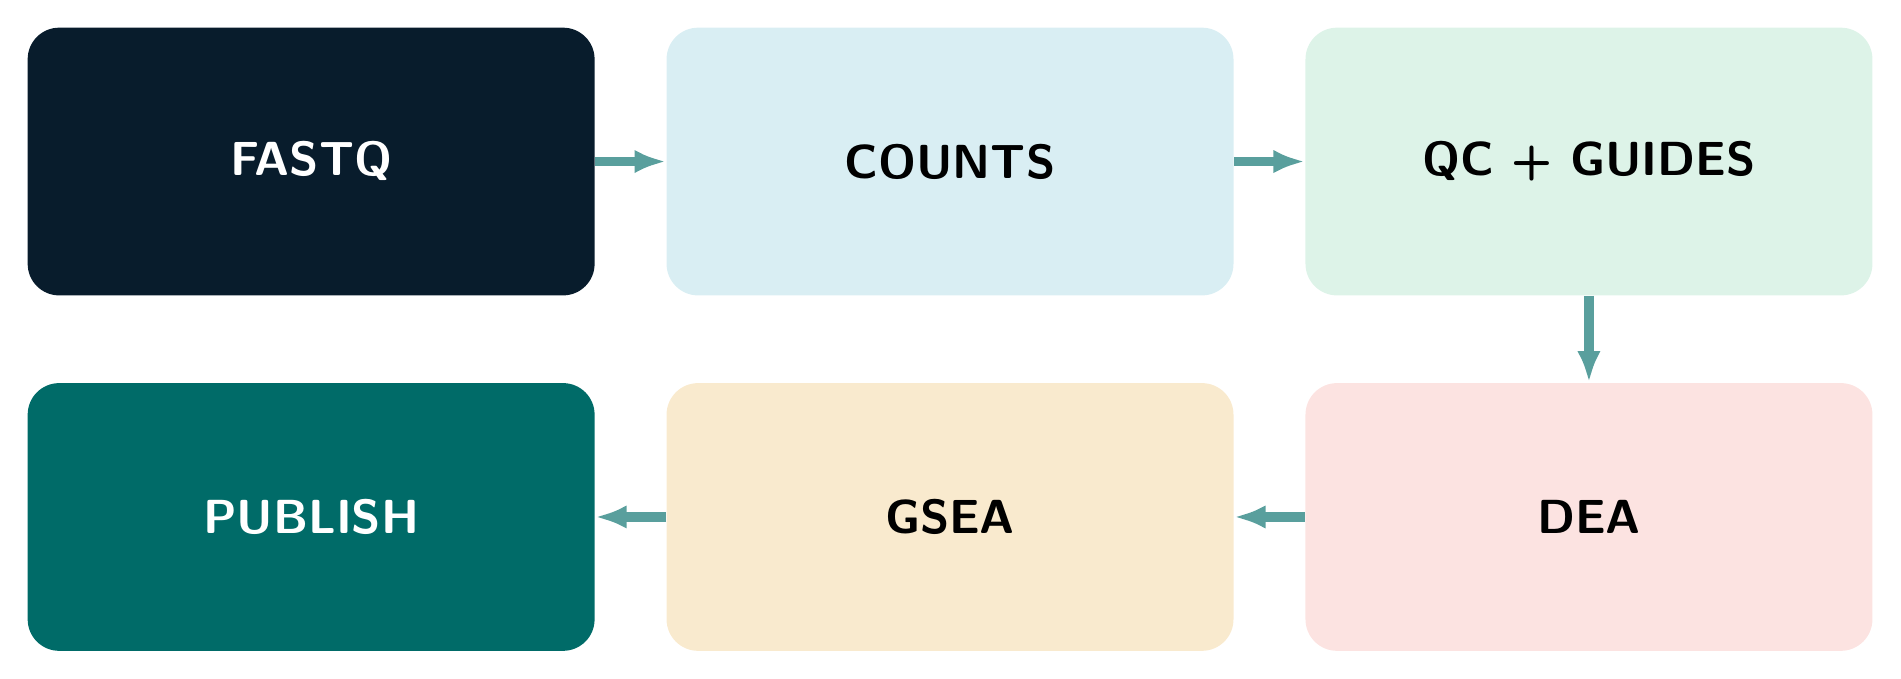
\begin{tikzpicture}[node distance=9mm]
      \node[rounded corners=4mm,fill=Navy,text=White,minimum width=72mm,
            minimum height=34mm,font=\fontsize{16}{18}\selectfont\bfseries] (f) {FASTQ};
      \node[right=9mm of f,rounded corners=4mm,fill=Sky,minimum width=72mm,
            minimum height=34mm,font=\fontsize{16}{18}\selectfont\bfseries] (c) {COUNTS};
      \node[right=9mm of c,rounded corners=4mm,fill=Mint,minimum width=72mm,
            minimum height=34mm,font=\fontsize{16}{18}\selectfont\bfseries] (q) {QC + GUIDES};
      \node[below=11mm of q,rounded corners=4mm,fill=Coral!18,minimum width=72mm,
            minimum height=34mm,font=\fontsize{16}{18}\selectfont\bfseries] (d) {DEA};
      \node[left=9mm of d,rounded corners=4mm,fill=Gold!28,minimum width=72mm,
            minimum height=34mm,font=\fontsize{16}{18}\selectfont\bfseries] (g) {GSEA};
      \node[left=9mm of g,rounded corners=4mm,fill=Teal,text=White,minimum width=72mm,
            minimum height=34mm,font=\fontsize{16}{18}\selectfont\bfseries] (p) {PUBLISH};
      \foreach \a/\b in {f/c,c/q,q/d,d/g,g/p}
        \draw[-{Latex[length=4mm,width=3mm]},line width=1.2mm,color=Teal!65] (\a) -- (\b);
    \end{tikzpicture}

    \vspace{10mm}
    \RaggedRight
    {\fontsize{18}{23}\selectfont
      \textcolor{Emerald}{\textbf{LIVE:}} Nadig 2025 (Jurkat, HepG2) + Replogle 2022
      (K562 essential, K562 genome-wide, RPE1 essential).}

    \vfill
    \begin{tcolorbox}[boxrule=0pt,arc=5mm,colback=Mint,left=7mm,right=7mm,top=5mm,bottom=5mm]
      {\fontsize{19}{23}\selectfont\bfseries\color{Teal}
      Standardised DEA + Hallmark GSEA are searchable beside the curated experimental context.}
    \end{tcolorbox}
  \end{tcolorbox}
\end{minipage}\hfill
\begin{minipage}[t]{0.525\linewidth}
  \sectionhead{Coral}{Evidence in context}
  \begin{tcolorbox}[enhanced,boxrule=0pt,arc=7mm,colback=White,
    left=10mm,right=10mm,top=8mm,bottom=8mm,height=215mm]
    {\fontsize{31}{34}\selectfont\bfseries\color{Navy}Search once. Traverse modalities.}\par
    \vspace{3mm}
    {\fontsize{18}{23}\selectfont\color{Slate}
      Find a target by symbol, synonym or Ensembl ID; see evidence across Perturb-Seq, CRISPR and MAVE.}
    \vspace{8mm}

    \centering
    \begin{tcolorbox}[enhanced,boxrule=.8mm,colframe=Line,colback=White,
      arc=5mm,left=2mm,right=2mm,top=2mm,bottom=2mm]
      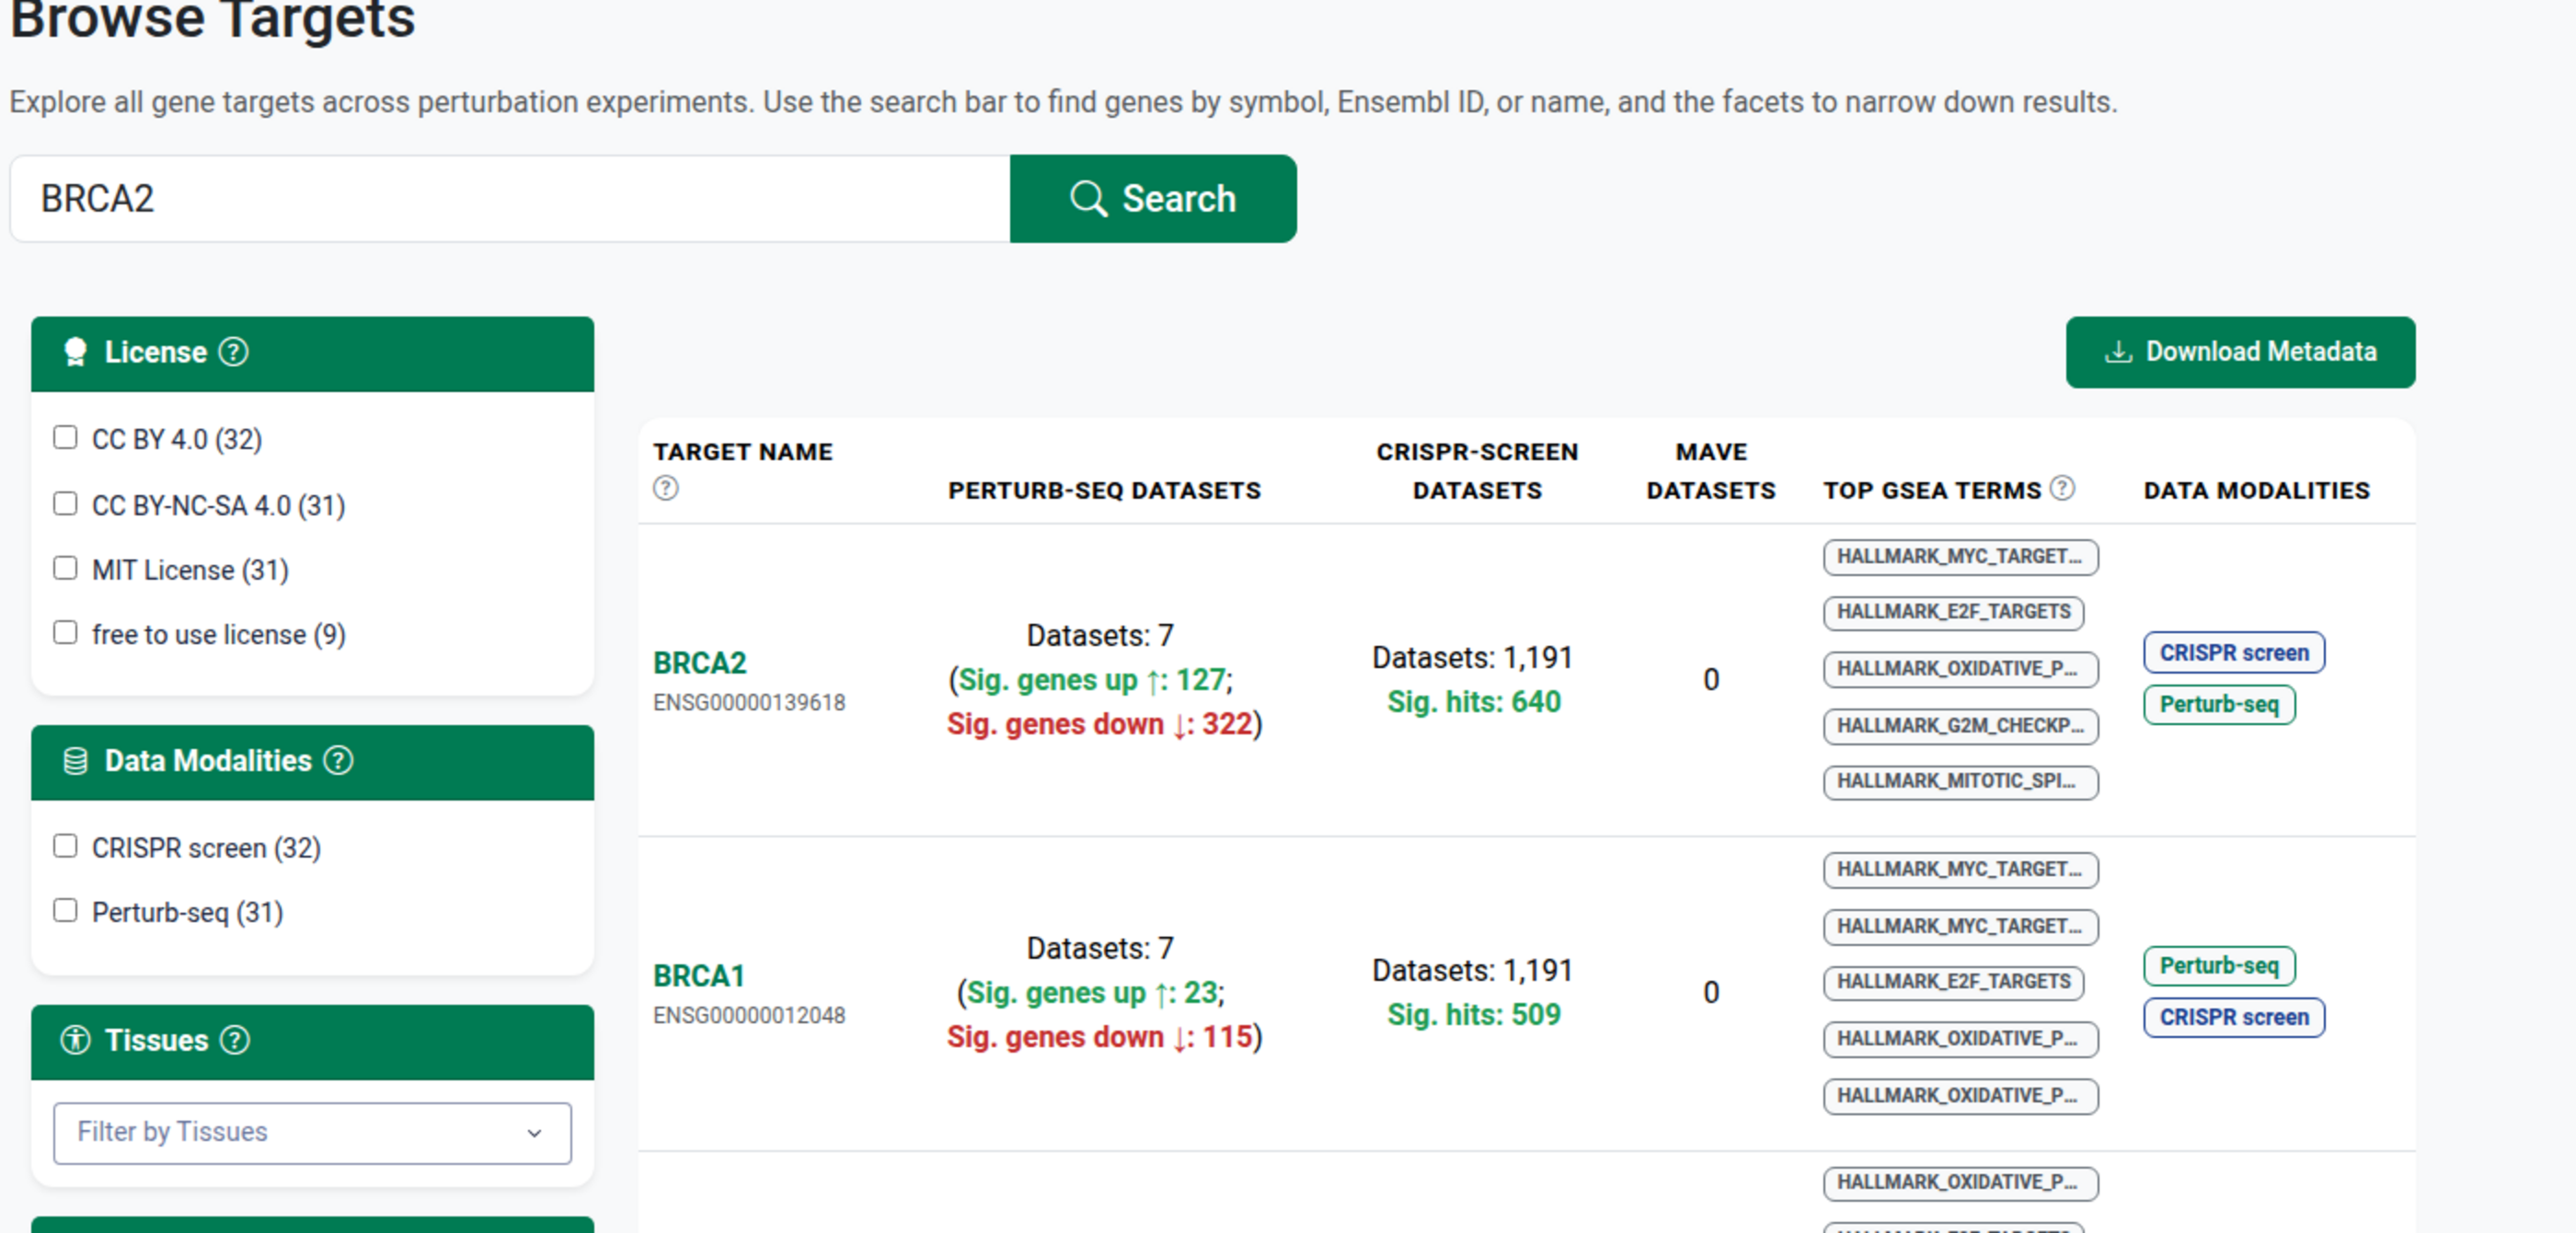
\includegraphics[width=\linewidth]{assets/target-search.png}
    \end{tcolorbox}

    \vspace{5mm}
    {\fontsize{16}{20}\selectfont\color{Slate}
      Live target browser shown for \textbf{BRCA2}: modality coverage, significant hits and top enriched pathways in one view.}
  \end{tcolorbox}
\end{minipage}

\vspace{7mm}

% Access + next ---------------------------------------------------------------
\sectionhead{Gold}{Take the data with you}
\begin{tcolorbox}[enhanced,boxrule=0pt,arc=7mm,colback=White,
  left=10mm,right=10mm,top=5mm,bottom=5mm]
  \begin{minipage}[c]{0.235\linewidth}\centering
    {\fontsize{29}{32}\selectfont\bfseries\color{Emerald}PORTAL}\par
    \vspace{2mm}{\fontsize{17}{21}\selectfont Browse targets + datasets}
  \end{minipage}\hfill
  \begin{minipage}[c]{0.235\linewidth}\centering
    {\fontsize{29}{32}\selectfont\bfseries\color{Cyan}REST API}\par
    \vspace{2mm}{\fontsize{17}{21}\selectfont Everything shown on the site}
  \end{minipage}\hfill
  \begin{minipage}[c]{0.235\linewidth}\centering
    {\fontsize{29}{32}\selectfont\bfseries\color{Coral}FULL DATA}\par
    \vspace{2mm}{\fontsize{17}{21}\selectfont Parquet + compressed CSV}
  \end{minipage}\hfill
  \begin{minipage}[c]{0.235\linewidth}\centering
    {\fontsize{29}{32}\selectfont\bfseries\color{Gold}METADATA}\par
    \vspace{2mm}{\fontsize{17}{21}\selectfont Downloadable JSON}
  \end{minipage}
\end{tcolorbox}

\vspace{6mm}
\begin{minipage}[t]{0.56\linewidth}
  \sectionhead{Emerald}{Next}
  \bighead{A living resource, not a one-off integration.}
  \vspace{3mm}
  \begin{tcolorbox}[enhanced,boxrule=0pt,arc=7mm,colback=Mint,
    left=9mm,right=9mm,top=7mm,bottom=7mm]
    {\fontsize{20}{25}\selectfont
      \textbf{AI-assisted metadata curation} with human review\\[3mm]
      \textbf{Broader modality-specific reanalysis} and validation\\[3mm]
      \textbf{Periodic, versioned data releases} with transparent provenance}
  \end{tcolorbox}
\end{minipage}\hfill
\begin{minipage}[t]{0.405\linewidth}
  \sectionhead{Coral}{Shape what comes next}
  \begin{tcolorbox}[enhanced,boxrule=0pt,arc=7mm,colback=Navy,
    left=9mm,right=9mm,top=8mm,bottom=8mm]
    {\fontsize{27}{30}\selectfont\bfseries\color{White}Bring your hard-to-integrate evidence.}\par
    \vspace{3mm}
    {\fontsize{17}{22}\selectfont\color{White}
      Suggest datasets or features---or fund a focused, multi-year collaboration around the modalities and questions that matter to your programme.}
    \vspace{6mm}

    \begin{minipage}[c]{0.46\linewidth}\centering
      {\setlength{\fboxsep}{3mm}\colorbox{White}{\color{Ink}\href{https://www.ebi.ac.uk/perturbation-catalogue/}{\qrcode[height=38mm]{https://www.ebi.ac.uk/perturbation-catalogue/}}}}\\[2mm]
      {\fontsize{14}{17}\selectfont\bfseries\color{White}EXPLORE}
    \end{minipage}\hfill
    \begin{minipage}[c]{0.46\linewidth}\centering
      {\setlength{\fboxsep}{3mm}\colorbox{White}{\color{Ink}\href{mailto:perturbation-catalogue-help@ebi.ac.uk}{\qrcode[height=38mm]{mailto:perturbation-catalogue-help@ebi.ac.uk}}}}\\[2mm]
      {\fontsize{14}{17}\selectfont\bfseries\color{White}CONTACT}
    \end{minipage}

    \vspace{5mm}
    {\fontsize{16}{19}\selectfont\bfseries\color{White}
      perturbation-catalogue-help@ebi.ac.uk}
  \end{tcolorbox}
\end{minipage}

\vspace{6mm}

% Footer ---------------------------------------------------------------------
\begin{tcolorbox}[enhanced,boxrule=0pt,arc=5mm,colback=White,
  left=9mm,right=9mm,top=5mm,bottom=5mm]
  \begin{minipage}[c]{0.28\linewidth}
    
\includegraphics[width=105mm]{assets/embl-ebi-logo.png}
  \end{minipage}\hfill
  \begin{minipage}[c]{0.39\linewidth}\centering
    {\fontsize{16}{20}\selectfont\color{Slate}
      Open resource \textbullet\ Public API \textbullet\ Downloadable data\\
      \href{https://www.ebi.ac.uk/perturbation-catalogue/}{ebi.ac.uk/perturbation-catalogue}}
  \end{minipage}\hfill
  \begin{minipage}[c]{0.28\linewidth}\RaggedLeft
    {\fontsize{13}{16}\selectfont\color{Slate}Supported by}\quad
    
\includegraphics[width=105mm]{assets/open-targets-logo.png}
  \end{minipage}
\end{tcolorbox}

\end{minipage}
\end{document}
